% +------------------------------------------------------------------------+
% | Reference manual page: Subdivision_method_3.tex
% +------------------------------------------------------------------------+
% | 03/01/2005   Le-Jeng Andy Shiue
% | Package: Subdivision_surface_3
% | 
\RCSdef{\RCSSubdivisionRev}{$Id$}
\RCSdefDate{\RCSSubdivisionDate}{$Date$}
% +------------------------------------------------------------------------+

\ccRefPageBegin

%%RefPage: end of header, begin of main body
% +------------------------------------------------------------------------+


\begin{ccRefClass}{Subdivision_method_3}

\ccDefinition

A subdivision method recursively refines a coarse mesh and 
generates an ever closer approximation to a smooth surface.
\ccClassTemplateName\ consists of four subdivision methods
and their refinement hosts. Each refinement host is a template 
function of a polyhedron class and a 
geometry policy class. It refines the connectivity of the
control mesh and computes the geometry of the refined mesh.
The geometry computation is dedicated to the custom
geometry policy. A geometry policy consists of functions 
that compute the new point based on the subdivision stencil.
A stencil defines the footprint (a submesh of the control mesh)
of a new point.

The four supported refinement hosts are the 
primal quadrilateral quadrisection (PQQ),
the primal triangle quadrisection (PTQ), 
the dual quadrilateral quadrisection (DQQ), 
and the $\sqrt{3}$ triangulation.
These refinements are respectively used in 
Catmull-Clark, Loop, Doo-Sabin and $\sqrt{3}$ subdivision.
%, which are also supported as template functions in \ccClassTemplateName .

\ccInclude{CGAL/Subdivision_method_3.h}

% +-----------------------------------+
\ccHeading{Refinement Host}
A refinement host is a template function of 
a polyhedron class and a geometry mask class. It refines
the input polyhedron, and computes new points through 
the geometry masks.
\ccc{Subdivision_method_3} supports four refinement hosts:
\ccc{PQQ}, \ccc{PTQ}, \ccc{DQQ} and \ccc{Sqrt3}.

\begin{ccTexOnly}
  \begin{center}
    \parbox{0.6\textwidth}{%
      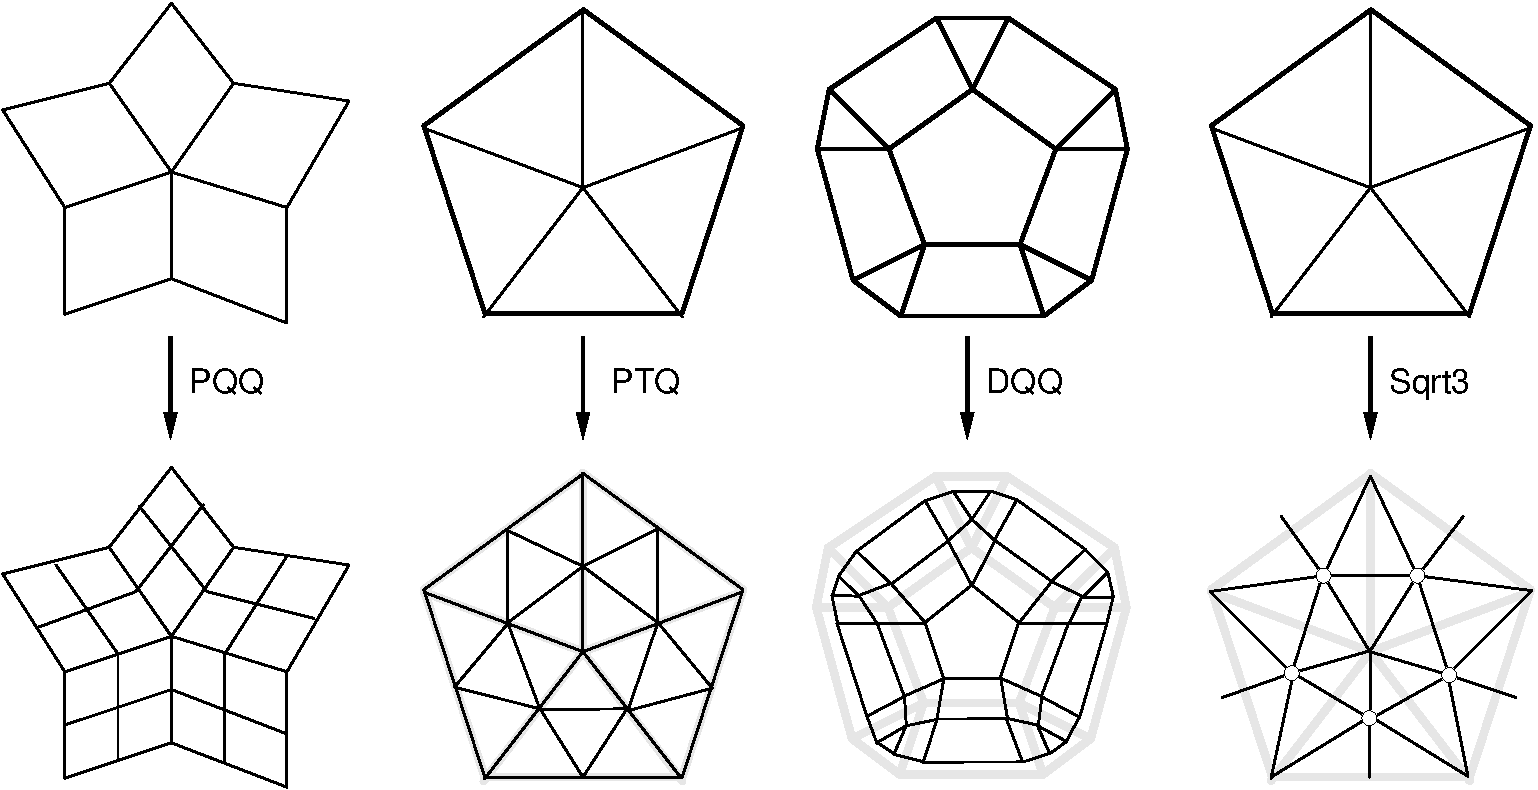
\includegraphics[width=0.6\textwidth]{Subdivision_method_3_ref/FIG/RefSchemes}%
    }\\ \vspace{0.5cm}
  \end{center}
\end{ccTexOnly}

\begin{ccHtmlOnly}
  <CENTER>
     <img src="FIG/RefSchemes.gif" alt="Refinement Hosts"><P>
  </CENTER>
\end{ccHtmlOnly}

\ccThree{void}{PQQ()}{}
\ccThreeToTwo

\ccFunction{
template <class Polyhedron_3, template <typename> class Mask>
void PQQ(Polyhedron_3& p, Mask<Polyhedron_3> mask, int step = 1);
}{
applies the PQQ refinement on the control mesh \ccc{p} \ccc{step} times.
The geometry of the refined mesh is computed by the geometry policy \ccc{mask}.
This function overwrites the control mesh \ccc{p} with the refined mesh.
}

\ccFunction{
template <class Polyhedron_3, template <typename> class Mask>
void PTQ(Polyhedron_3& p, Mask<Polyhedron_3> mask, int step = 1);
}{
applies the PTQ refinement on the control mesh \ccc{p} \ccc{step} times,
where \ccc{p} contains only triangle facets.
The geometry of the refined mesh is computed by the geometry policy \ccc{mask}.
This function overwrites the control mesh \ccc{p} with the refined mesh.
The result of a non-triangle mesh \ccc{p} is undefined.
}

\ccFunction{
template <class Polyhedron_3, template <typename> class Mask>
void DQQ(Polyhedron_3& p, Mask<Polyhedron_3> mask, int step = 1);
}{
applies the DQQ refinement on the control mesh \ccc{p} \ccc{step} times.
The geometry of the refined mesh is computed by the geometry policy \ccc{mask}.
This function overwrites the control mesh \ccc{p} with the refined mesh.
}

\ccFunction{
template <class Polyhedron_3, template <typename> class Mask>
void Sqrt3(Polyhedron_3& p, Mask<Polyhedron_3> mask, int step = 1);
}{
applies the $\sqrt{3}$ triangulation on the control mesh \ccc{p} 
\ccc{step} times, where \ccc{p} contains only triangle facets.
The geometry of the refined mesh is computed by the geometry policy \ccc{mask}.
This function overwrites the control mesh \ccc{p} with the refined mesh.
The result of a non-triangle mesh \ccc{p} is undefined.
}

% +-----------------------------------+
\ccHeading{Subdivision Method}

%\ccTwo{void CatmullClark_subdivision(Poly& p, int d);}{}
\ccThree{void}{sub}{}
\ccThreeToTwo

\ccFunction{
template <class Polyhedron_3>
void CatmullClark_subdivision(Polyhedron_3& p, int step = 1);
}{
applies Catmull-Clark subdivision \ccc{step} times on the control mesh \ccc{p}.
This function overwrites the control mesh \ccc{p} with the subdivided mesh.
}

\ccFunction{
template <class Polyhedron_3>
void Loop_subdivision(Polyhedron_3& p, int step = 1); 
}{
applies Loop subdivision \ccc{step} times on the control mesh \ccc{p}.
This function overwrites the control mesh \ccc{p} with the subdivided mesh.
}

\ccFunction{
template <class Polyhedron_3>
void DooSabin_subdivision(Polyhedron_3& p, int step = 1);
}{
applies Doo-Sabin subdivision \ccc{step} times on the control mesh \ccc{p}.
This function overwrites the control mesh \ccc{p} with the subdivided mesh.
}

\ccFunction{
template <class Polyhedron_3>
void Sqrt3_subdivision(Polyhedron_3& p, int step = 1);
}{
applies $\sqrt{3}$ subdivision \ccc{step} times on the control mesh \ccc{p}.
This function overwrites the control mesh \ccc{p} with the subdivided mesh.
}

\ccSeeAlso

%\ccRefIdfierPage{CGAL::PQQ_stencil_3<Polyhedron_3>}\\
%\ccRefIdfierPage{CGAL::DQQ_stencil_3<Polyhedron_3>}\\
%\ccRefIdfierPage{CGAL::Linear_mask_3<Polyhedron_3>}\\
\ccRefIdfierPage{CGAL::CatmullClark_mask_3<Polyhedron_3>}\\
\ccRefIdfierPage{CGAL::Loop_mask_3<Polyhedron_3>}\\
\ccRefIdfierPage{CGAL::Sqrt3_mask_3<Polyhedron_3>}\\

\ccExample

This example program subdivides a polyhedral mesh with
Catmull-Clark subdivision.

\ccIncludeExampleCode{Subdivision_method_3/CatmullClark_subdivision.cpp}

\end{ccRefClass}

% +------------------------------------------------------------------------+
%%RefPage: end of main body, begin of footer
\ccRefPageEnd
% EOF
% +------------------------------------------------------------------------+
